\clearpage

\section{Introduction}

Heavy quarks nuclear modification factor ($R_{AA}$) has been proposed as an important measurement to study the flavor dependence of partons energy loss in the medium, and eventually to help in extracting the medium transport, drag and diffusion coefficients. There are lots of theoretical calculations for the energy losses for different flavor particles. Fig.~\ref{fig:raa_CUJE} shows the jet flavor tomography level crossing pattern of nuclear modification factors at middle rapidity of $\pi$, D, B, e from CUJT calculations for central Au + Au 200 GeV collisions. As clearly see the mass hierarchy of the different flavor energy loss.

The hadronic channels allow to fully reconstruct the charmed hadrons and do not suffer from the complications in the semi-leptonic decays, however the measurement can be challenging due to large combinatorial backgrounds and lower branching ratios. One approach is to use the decay topology to reduce this background by distinguishing between tracks that come from the collision itself (primary vertex) and those from a secondary decay vertex. This requires the detectors must be able to resolve differences on the order of tens of microns. Heavy Flavor Tracker (HFT) is essence the right detector for this mission.

Fig.~\ref{fig:BeforeHFT} shows the $R_{AA}$ of $D^0$, $\pi$, $h^{\pm}$ from various measurements. A significant suppression is clearly seen at the high $p_T$ range for both light hadrons and charmed hadrons both in RHIC energy and LHC energy. The enhancement observed in the intermediate $p_T$ range from STAR can be described by the models including coalescence of charm and light quarks, even though the uncertainties are still large in the low transverse momentum range. It will be critical to precise measure the low $p_T$ structure.

\begin{figure}
\centering
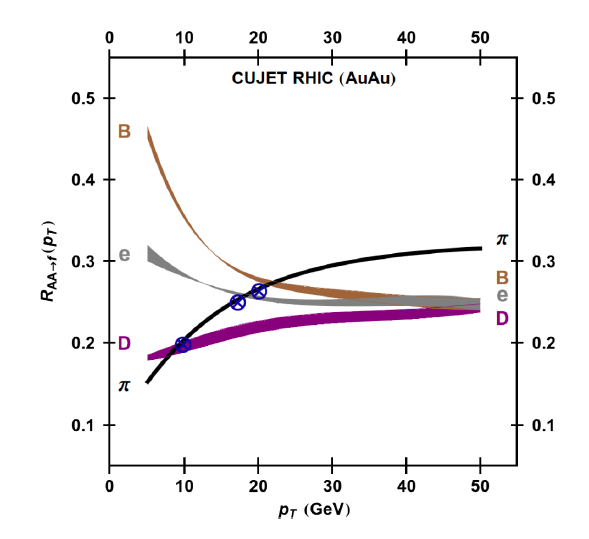
\includegraphics[width=0.45\textwidth]{figure/Run14_D0HFT/raa_CUJE.png}
\caption{Jet flavor tomography level crossing pattern of nuclear modification factors at middle rapidity of $\pi$, D, B, e calculations for central Au + Au 200 GeV collisions.}
\label{fig:raa_CUJE} 
\end{figure}

\begin{figure}
\centering
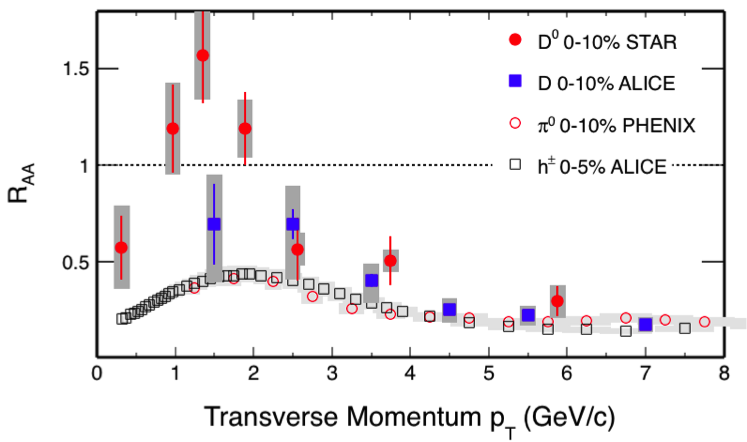
\includegraphics[width=0.5\textwidth]{figure/Run14_D0HFT/BeforeHFT.png}
\caption{(upper) $D^0$, $\pi$, $h^{\pm}$ $R_{AA}$ from different measurements. (bottom) $v_2$ of $D$ and $h^{\pm}$ from ALICE.}
\label{fig:BeforeHFT} 
\end{figure}